\documentclass[11pt,a4paper]{article}

\usepackage[T1]{fontenc}
\usepackage[utf8]{inputenc}
\usepackage{lmodern}
\usepackage[margin=2.5cm]{geometry}
\usepackage{amsmath,amssymb,amsthm}
\usepackage{mathtools}
\usepackage{microtype}
\usepackage{booktabs}
\usepackage{array}
\usepackage{enumitem}
\usepackage{xcolor}
\usepackage{algorithm}
\usepackage[noend]{algpseudocode}
\usepackage{pgfplots}
\usepgfplotslibrary{groupplots}
\pgfplotsset{compat=1.17}
\usepackage[colorlinks=true,linkcolor=blue!50!black,citecolor=green!40!black,urlcolor=blue!50!black]{hyperref}
\usepackage[capitalise,noabbrev]{cleveref}

% ---------- theorem environments ----------
\theoremstyle{plain}
\newtheorem{theorem}{Theorem}
\newtheorem{lemma}[theorem]{Lemma}
\newtheorem{proposition}[theorem]{Proposition}
\newtheorem{corollary}[theorem]{Corollary}
\newtheorem{conjecture}[theorem]{Conjecture}
\theoremstyle{definition}
\newtheorem{definition}[theorem]{Definition}
\theoremstyle{remark}
\newtheorem{remark}[theorem]{Remark}
\crefname{conjecture}{Conjecture}{Conjectures}

% ---------- macros ----------
\newcommand{\todo}[1]{\textcolor{red!75!black}{\textbf{[#1]}}}
\newcommand{\far}{\mathrm{far}_r}
\newcommand{\per}{\mathrm{per}}
\newcommand{\ccw}{\textsc{ccw}}
\DeclareMathOperator{\conv}{conv}
\newcommand{\rs}{r^{*}}
\newcommand{\Tr}{T_r}
\newcommand{\Oh}{O}
\newcommand{\circleof}{\bigcirc}

\title{Exact $k$-Dispersion for Points in Convex Position:\\
a Capped Delaunay Dynamic Program and the Limits of Greedy Structure}
\author{\todo{Author names}\\ \small\todo{Affiliations and e-mail addresses}}
\date{\todo{Date of submission}}

\begin{document}
\maketitle

\begin{abstract}
Given $n$ points in convex position in the plane and an integer $k$, the
$k$-dispersion problem asks for $k$ of the points whose minimum pairwise distance
$\rs$ is as large as possible. The best previously known deterministic algorithm
runs in $\Oh(n^3\log^2 n)$ time (Tkachenko and Wang, SWAT~2026). We give an exact
algorithm running in $\Oh(n^3\log k\log n)$ time and $\Oh(n^2k)$ space. Its decision
procedure takes $\Oh(n^2k+\Tr\log k)\subseteq\Oh(n^3\log k)$ time, where $\Tr$ is the
number of triples of pairwise $r$-far points. It is a dynamic program over
triangulations that stores only $k-2$ apex points per chord and uses only exact
orientation and in-circle predicates on integers. Its correctness rests on a
\emph{Delaunay certificate}: a set in convex position has all pairwise distances at
least $r$ if and only if it has a triangulation whose edges all have length at
least $r$ and whose diagonals are all locally Delaunay.

We also study whether greedy structure can give faster algorithms for $k\ge 4$. The
arc characterisation behind the near-linear algorithm for $k=3$ fails for every
$4\le k\le 6$ on explicit, exhaustively verified instances, and so do several
natural seeded greedy rules. A ``tight-pair'' property and a search-tree
strengthening of it survived more than $1.3$ million exact tests; we state both as
conjectures. The second would yield an $\Oh(2^kn^2k\log n)$ algorithm. Finally, a
\emph{certified} variant runs an $\Oh(n^2k)$ greedy and then makes one exact decision.
It always returns the optimum, and it runs in $\Oh(n^2k\log n+n^3\log k)$ time
whenever the greedy value is optimal, which was the case on all large test instances.
All algorithms were implemented and cross-checked against exhaustive search.
\end{abstract}

% ======================================================================
\section{Introduction}\label{sec:intro}

Let $P$ be a set of $n$ points in the plane in \emph{convex position}, that is,
every point of $P$ is a vertex of the convex hull $\conv(P)$. For an integer
$2\le k\le n$, the \emph{$k$-dispersion} problem (also called max--min dispersion
or the maximally separated set problem) asks for a subset $S\subseteq P$ with $|S|=k$
that maximises
\[
  \delta(S)=\min_{p\neq q\in S}|pq|.
\]
We write $\rs=\rs_k(P)$ for the optimum. Dispersion models facility location with
mutually obnoxious facilities, such as shops of one chain or hazardous plants, and
the selection of diverse representatives~\cite{RRT94}. For general planar point
sets the problem is NP-hard~\cite{WK88}. The best exact algorithms run in
$n^{\Oh(\sqrt k)}$~\cite{Akagi18} or $\Oh(n^{k-1}\log n)$ time~\cite{CD25}, and a
generic approach finds a $k$-clique in the threshold graph by fast matrix
multiplication~\cite{NP85,EG04}. Convex position makes the problem polynomial.

\paragraph{Known results.}
\Cref{tab:known} summarises the exact algorithms for convex position that we are
aware of.

\begin{table}[ht]
\centering
\caption{Exact algorithms for $k$-dispersion of $n$ points in convex position.}
\label{tab:known}
\small
\begin{tabular}{@{}l>{$}l<{$}p{5.6cm}@{}}
\toprule
Reference & \text{Time} & Remarks\\
\midrule
Singireddy, Basappa, Mitchell~\cite{SBM26} & \Oh(2^kn^2\log^2 n) & bounded search tree, FPT in $k$\\
Singireddy, Basappa, Mitchell~\cite{SBM26} & \Oh(n^4k^2) & first polynomial algorithm\\
Tkachenko, Wang~\cite{TW25} & \Oh(n^{7/2}\log n) & randomised: $\Oh(n^{37/11}\log n)$ expected\\
Tkachenko, Wang~\cite{TW26} & \Oh(n^3\log^2 n) & via $\Oh(n^3\log n)$ maximum independent set\\
Kobayashi et al.~\cite{Kob22} & \Oh(n^2) & $k=3$\\
Tkachenko, Wang~\cite{TW25} & \Oh(n\log^2 n) & $k=3$; $\Oh(n\log n)$ expected\\
\midrule
This paper (\cref{thm:opt}) & \Oh(n^3\log k\log n) & decision in $\Oh(n^3\log k)$, integer predicates\\
This paper (\cref{thm:certified}) & \Oh(n^2k\log n+n^3\log k) & when the greedy value is optimal; always exact\\
\bottomrule
\end{tabular}
\end{table}

\paragraph{Contributions.}
\begin{enumerate}[leftmargin=*,label=(\arabic*)]
\item \emph{A Delaunay certificate (\cref{thm:cert}).} A set $S$ in convex position
  is $r$-far (all pairwise distances at least $r$) if and only if $S$ has a
  triangulation in which every edge has length at least $r$ and every diagonal is
  locally Delaunay. The two ingredients are classical. Their combination makes both
  conditions \emph{local}. This allows a dynamic program and replaces the
  seven-term distance inequality used in the correctness proof of~\cite{TW25}.
\item \emph{A capped Delaunay dynamic program (\cref{sec:dp}).} The value of a chord
  in the dynamic program depends on an angle bound inherited from its parent, so it
  is a step function of that angle. A decision only asks whether $k$ points fit,
  so it suffices to store the first $k-2$ steps of this function
  (\cref{lem:thresholds}), each represented by an input point. This yields an
  exact decision procedure in $\Oh(n^2k+\Tr\log k)$ time and $\Oh(n^2k)$ space that
  uses only orientation and in-circle tests (\cref{thm:decision}), and an
  $\Oh(n^3\log k\log n)$-time algorithm for the optimisation problem
  (\cref{thm:opt}). No cuttings or other geometric data structures are needed.
\item \emph{A search window (\cref{lem:window}).}
  $g\le\rs\le\min\{2g,\per(P)/k\}$, where $g$ is the value of the farthest-first
  greedy $k$-set and $\per(P)$ is the perimeter of $\conv(P)$. The bound
  $\rs\le 2g$ is the classical 2-approximation guarantee~\cite{RRT94,Gon85}. The
  perimeter bound is new to our knowledge. In experiments the window keeps a median
  of $6.3\%$ of the candidate distances.
\item \emph{Greedy structure (\cref{sec:greedy}).} The arc characterisation behind
  the algorithms for $k=3$~\cite{Kob22,TW25} fails for $k=4,5,6$, and several
  natural seeded greedy rules are incomplete. We give minimal counterexamples with
  $6$, $8$ and $10$ points. Two properties survived all of more than $1.3$ million
  exact tests, and we state them as \cref{conj:tight,conj:tree}.
\item \emph{A certified algorithm (\cref{thm:certified}) and experiments
  (\cref{sec:exp}).} All algorithms were implemented and cross-checked against
  exhaustive search, an independent dynamic program and a generic
  matrix-multiplication-based solver.
\end{enumerate}

\paragraph{Positioning.}
Our worst-case bound $\Oh(n^3\log k\log n)$ improves on $\Oh(n^3\log^2 n)$~\cite{TW26}
by a factor $\log n/\log k$, which is unbounded when $k=n^{o(1)}$. It is also at most
the FPT bound $\Oh(2^kn^2\log^2 n)$~\cite{SBM26} whenever $2^k\log n\ge n\log k$, in
particular whenever $k\ge\log_2 n$. It is therefore the best known deterministic
bound for $\log_2 n\le k\le n^{o(1)}$. Our decision bound $\Oh(n^3\log k)$ likewise
improves the $\Oh(n^3\log n)$ decision bound implied by~\cite{TW26} when $k=n^{o(1)}$.
The subproblems of our dynamic program are, in substance, those of~\cite{TW25}. What
is new is the certificate-based correctness proof, the $k$-capped threshold
representation, the predicate-only implementation, the perimeter window, and the
structural results of \cref{sec:greedy}. \todo{Compare with the techniques of
\cite{TW26} in detail once its full text has been checked; in particular, state
whether it already uses a capped representation.}

\paragraph{Organisation.}
\Cref{sec:prelim} fixes notation and the model of computation.
\Cref{sec:cert} proves the certificate, \cref{sec:dp} develops the capped dynamic
program, and \cref{sec:opt} derives the optimisation algorithm and the search
window. \Cref{sec:greedy} studies greedy structure and gives the certified
algorithm. \Cref{sec:exp} reports experiments and \cref{sec:open} lists open
problems.

% ======================================================================
\section{Preliminaries}\label{sec:prelim}

\begin{table}[ht]
\centering
\caption{Notation.}\label{tab:notation}
\begin{tabular}{@{}>{$}l<{$}p{0.74\textwidth}@{}}
\toprule
P=(p_0,\dots,p_{n-1}) & input points in strictly convex position, in counterclockwise (\ccw) order; indices are taken mod $n$\\
|pq|,\ D(i,j) & Euclidean distance; squared distance $|p_ip_j|^2$ (an integer)\\
P(i,j) & the points strictly between $p_i$ and $p_j$, going \ccw\ from $p_i$\\
\text{$r$-far} & a set whose pairwise distances are all at least $r$\\
\far(i,j) & the predicate $|p_ip_j|\ge r$\\
\angle abc & the angle at $b$ in the triangle $abc$, in $(0,\pi)$\\
\circleof(a,b,c) & the circle through $a$, $b$, $c$\\
a(q),\ b(q) & the first point \ccw\ (respectively clockwise) from $q$ at distance at least $r$\\
F(i,j\mid\varphi) & value of chord $(i,j)$ under apex-angle bound $\varphi$ (\cref{def:config})\\
\tau_c(i,j),\ L_c(i,j) & $c$-th threshold angle of chord $(i,j)$ and an apex attaining it (\cref{lem:thresholds}); $K=k-2$\\
\Tr & number of \ccw\ triples $(i,l,j)$ with $\far(i,l)$, $\far(l,j)$ and $\far(i,j)$\\
\per(P) & perimeter of $\conv(P)$\\
\bottomrule
\end{tabular}
\end{table}

A \emph{triangulation} of a finite set $S$ in convex position is a maximal set of
pairwise non-crossing segments (\emph{edges}) between points of $S$. Its edges are
the hull sides of $S$ and the \emph{diagonals}. A diagonal $ab$ with incident
triangles $abc$ and $bad$ is \emph{locally Delaunay} if $d$ does not lie strictly
inside $\circleof(a,b,c)$. Since $acbd$ is a convex quadrilateral, this is
equivalent to $\angle acb+\angle adb\le\pi$. A triangulation is \emph{Delaunay} if no
point of $S$ lies strictly inside the circumcircle of any of its triangles.

\paragraph{Model of computation and exact predicates.}
Input coordinates are integers of absolute value at most $2^{29}$. Then coordinate
differences have absolute value at most $2^{30}$, squared distances are at most
$2^{61}$, and the orientation determinant has absolute value at most $2^{61}$. The
in-circle determinant, written as a $3\times3$ determinant of translated
coordinates and expanded along its lifted column, has absolute value at most
$3\cdot2^{61}\cdot2^{61}<2^{124}$. All
predicates are therefore evaluated exactly in signed 128-bit integer arithmetic, with
no floating point and no rounding~\cite{Shewchuk97}. Every angle comparison in this
paper reduces to these predicates through two classical facts.
\begin{enumerate}[label=(P\arabic*)]
\item\label{P1} For points $x,y$ on the same side of the line $p_ip_j$,
  $\angle p_ixp_j>\angle p_iyp_j$ if and only if $x$ lies strictly inside
  $\circleof(p_i,y,p_j)$ (inscribed angle theorem).
\item\label{P2} For a convex quadrilateral with vertices $p_i,x,p_l,p_j$ in this
  order, $\angle p_ixp_l+\angle p_ip_jp_l>\pi$ if and only if $x$ lies strictly inside
  $\circleof(p_i,p_l,p_j)$. Equality holds exactly when the four points are
  concyclic, because opposite angles of a cyclic quadrilateral sum to $\pi$.
\end{enumerate}

% ======================================================================
\section{A Delaunay certificate for \texorpdfstring{$r$}{r}-far sets}\label{sec:cert}

\begin{lemma}[Delaunay lemma~\cite{Del34,Ede01,BCKO08}]\label{lem:delaunay}
If every diagonal of a triangulation $T$ of a finite point set $S$ is locally
Delaunay, then $T$ is a Delaunay triangulation of $S$.
\end{lemma}

\begin{lemma}[closest pairs are Delaunay edges; classical, see~{\cite[Ch.~9]{BCKO08}}]\label{lem:closest}
Let $S$ be a finite point set, not all on a line, and let $T$ be any Delaunay
triangulation of $S$. Then $\min_{p\neq q\in S}|pq|$ is the length of an edge of $T$.
\end{lemma}

\begin{proof}
Let $p,q$ be a closest pair and let $D$ be the closed disk with diameter $pq$.
Suppose some $s\in S\setminus\{p,q\}$ lies in $D$. Then $\angle psq\ge\pi/2$, so
$|pq|^2\ge|ps|^2+|sq|^2>|ps|^2$, which contradicts the minimality of $|pq|$. Hence
the boundary circle of $D$ passes through $p$ and $q$, and $D$ contains no other
point of $S$. Therefore $pq$ is an edge of the Delaunay graph of $S$. Every Delaunay
triangulation contains the Delaunay graph, because it is obtained by triangulating
the faces of the graph~\cite[Ch.~9]{BCKO08}.
\end{proof}

\begin{theorem}[Delaunay certificate]\label{thm:cert}
Let $S$ be in strictly convex position, $|S|\ge3$, and $r>0$. Then $S$ is $r$-far
if and only if $S$ has a triangulation $T$ such that
\begin{enumerate}[label=(\alph*)]
  \item every edge of $T$ has length at least $r$, and
  \item every diagonal of $T$ is locally Delaunay.
\end{enumerate}
\end{theorem}

\begin{proof}
($\Leftarrow$) By \cref{lem:delaunay}, $T$ is Delaunay. By \cref{lem:closest}, the
minimum pairwise distance in $S$ equals the minimum edge length of $T$, which is at
least $r$.
($\Rightarrow$) Any Delaunay triangulation of $S$ satisfies~(b). All its edges join
points of $S$, so~(a) holds because $S$ is $r$-far.
\end{proof}

Both conditions are \emph{local}: (a) concerns single edges and (b) concerns single
pairs of adjacent triangles. This is what makes a dynamic program possible. The
algorithm of Tkachenko and Wang~\cite{TW25} has a similar structure, but its
correctness proof uses a seven-term distance inequality (their Lemma~14).
\Cref{thm:cert} gives a shorter route that uses only textbook facts.

% ======================================================================
\section{The capped Delaunay dynamic program}\label{sec:dp}

Fix $r$ and write $\mathrm{far}$ for $\far$. A chord $(i,j)$ is \emph{admissible}
if $\mathrm{far}(i,j)$ holds. A point $p_l\in P(i,j)$ is an \emph{admissible apex}
of $(i,j)$ if $\mathrm{far}(i,l)$ and $\mathrm{far}(l,j)$ hold.

\begin{definition}\label{def:config}
For an admissible chord $(i,j)$, an \emph{$(i,j)$-configuration} is a pair $(X,T)$
where $X\subseteq P(i,j)$ and $T$ is a triangulation of $X\cup\{p_i,p_j\}$ such that
(a)~all edges of $T$ have length at least $r$ and (b)~all diagonals of $T$ are
locally Delaunay. If $X\neq\emptyset$, the \emph{apex} of $(X,T)$ is the third vertex
$p_l$ of the triangle of $T$ that contains the edge $p_ip_j$. For
$\varphi\in(0,\pi]$, let $F(i,j\mid\varphi)$ be the maximum of $|X|$ over all
configurations with $X=\emptyset$ or $\angle p_ip_lp_j\le\varphi$.
\end{definition}

The bound $\varphi$ encodes the parent. Suppose $p_ip_j$ becomes a diagonal whose
other triangle is $p_jp_ip_t$. Then $p_ip_j$ is locally Delaunay exactly when
$\angle p_ip_lp_j\le\pi-\angle p_ip_tp_j$.

\begin{lemma}[recurrence]\label{lem:rec}
For every admissible chord $(i,j)$ and every $\varphi\in(0,\pi]$,
\begin{multline*}
  F(i,j\mid\varphi)=\max\Bigl(\{0\}\cup\bigl\{\,1+F(i,l\mid\pi-\angle p_ip_jp_l)
  +F(l,j\mid\pi-\angle p_lp_ip_j) \;:\\ l\text{ admissible apex},\ \angle p_ip_lp_j\le\varphi\,\bigr\}\Bigr).
\end{multline*}
\end{lemma}

\begin{proof}
($\ge$) Take an admissible apex $l$ with $\angle p_ip_lp_j\le\varphi$. Take optimal
configurations $(X_1,T_1)$ for $(i,l)$ and $(X_2,T_2)$ for $(l,j)$ under the stated
bounds. Let $X=X_1\cup X_2\cup\{p_l\}$ and $T=T_1\cup T_2\cup\{p_ip_lp_j\}$. The new
edges $p_ip_l$, $p_lp_j$ and $p_ip_j$ have length at least $r$. If
$X_1\neq\emptyset$, then $p_ip_l$ is a diagonal of $T$ between the triangle
$p_ip_lp_j$ and the apex triangle of $T_1$, and the bound
$\pi-\angle p_ip_jp_l$ is exactly its local Delaunay condition. The same holds
symmetrically for $p_lp_j$. Every other diagonal of $T$ is a diagonal of $T_1$ or
$T_2$. The apex of $(X,T)$ is $p_l$, and $\angle p_ip_lp_j\le\varphi$.
($\le$) Let $(X,T)$ be an optimal configuration with $X\neq\emptyset$, and let $p_l$
be its apex. Removing the triangle $p_ip_lp_j$ splits $T$ into configurations for
$(i,l)$ and $(l,j)$. Both chords have length at least $r$ by~(a), so $l$ is an
admissible apex. By~(b), the apex angles of the two parts obey the stated bounds.
Hence $|X|\le1+F(i,l\mid\cdot)+F(l,j\mid\cdot)$.
\end{proof}

\begin{theorem}[decision]\label{thm:dec-char}
Let $k\ge3$. Then $P$ has an $r$-far $k$-set if and only if some admissible chord
$(i,j)$ has $F(i,j\mid\pi)\ge k-2$.
\end{theorem}

\begin{proof}
($\Rightarrow$) Let $S=\{q_1,\dots,q_k\}$ be $r$-far, in \ccw\ order, and let $T$ be
a Delaunay triangulation of $S$. Let $p_i=q_1$, $p_j=q_k$ and
$X=S\setminus\{q_1,q_k\}\subseteq P(i,j)$. By \cref{thm:cert}($\Rightarrow$),
$(X,T)$ is an $(i,j)$-configuration. Its apex angle is less than $\pi$, so
$F(i,j\mid\pi)\ge k-2$.
($\Leftarrow$) A configuration with $|X|\ge k-2$ is a triangulation of
$X\cup\{p_i,p_j\}$ that satisfies (a) and~(b). By \cref{thm:cert} this set is
$r$-far, and any $k$ of its points form the required set.
\end{proof}

\subsection{Thresholds: only \texorpdfstring{$k-2$}{k-2} numbers per chord}

Fix an admissible chord $(i,j)$. For an admissible apex $l$, let
$v(l)=1+F(i,l\mid\pi-\angle p_ip_jp_l)+F(l,j\mid\pi-\angle p_lp_ip_j)$. For $c\ge1$,
let
\[
  \tau_c(i,j)=\min\{\angle p_ip_lp_j : l \text{ admissible},\ v(l)\ge c\},
\]
with $\tau_c(i,j)=+\infty$ if no such $l$ exists, and let $\tau_0=0$.

\begin{lemma}\label{lem:thresholds}
$\tau_1(i,j)\le\tau_2(i,j)\le\cdots$ and $F(i,j\mid\varphi)=\max\{c\ge0:\tau_c(i,j)\le\varphi\}$.
Moreover, let $K=k-2$ and $F_K=\min(F,K)$. Then the values $\tau_1,\dots,\tau_K$ of
every chord are determined by the values $F_K$ of shorter chords.
\end{lemma}

\begin{proof}
The sets $\{l:v(l)\ge c\}$ shrink as $c$ grows, which gives monotonicity. By
\cref{lem:rec}, $F(i,j\mid\varphi)\ge c$ holds if and only if some admissible $l$ with
$\angle p_ip_lp_j\le\varphi$ has $v(l)\ge c$, that is, if and only if
$\tau_c\le\varphi$. For the last claim, note that
$\min(K,v(l))=\min\bigl(K,1+F_K(i,l\mid\cdot)+F_K(l,j\mid\cdot)\bigr)$, and that
$\tau_c$ for $c\le K$ depends on $v$ only through $\min(K,v)$.
\end{proof}

We store $\tau_c(i,j)$ as an apex point $L_c(i,j)$ that attains it, and write
$L_c(i,j)=\bot$ if $\tau_c(i,j)=+\infty$. By \cref{lem:thresholds} and~\ref{P2}, the
query $F_K(i,l\mid\pi-\angle p_ip_jp_l)\ge c$ becomes ``$L_c(i,l)\neq\bot$ and
$L_c(i,l)$ is not strictly inside $\circleof(p_i,p_l,p_j)$''. This condition is
monotone in $c$, so the number of values of $c$ that satisfy it can be found by
binary search with $\Oh(\log K)$ in-circle tests. By~\ref{P1}, comparing apex angles
is also an in-circle test.

\begin{algorithm}[ht]
\caption{\textsc{CappedDecision}$(P,k,r)$ for $k\ge3$; $K=k-2$}\label{alg:capped}
\begin{algorithmic}[1]
\For{$s=2,\dots,n-1$} \Comment{chords in order of increasing \ccw\ gap}
  \For{each admissible chord $(i,j)$ with $j=i+s$}
    \State $\mathit{best}[1..K]\gets\bot$
    \For{each admissible apex $p_l\in P(i,j)$}
      \State $q_1\gets\#\{c\le K: L_c(i,l)\ne\bot$, not strictly inside $\circleof(p_i,p_l,p_j)\}$ \Comment{bin.\ search}
      \State $q_2\gets\#\{c\le K: L_c(l,j)\ne\bot$, not strictly inside $\circleof(p_i,p_l,p_j)\}$
      \State $v\gets\min(K,1+q_1+q_2)$; store $p_l$ in $\mathit{best}[v]$ if its apex angle is smaller
    \EndFor
    \State $L_c(i,j)\gets$ smallest-angle apex in $\mathit{best}[c..K]$, $c=K,\dots,1$ \Comment{suffix minima}
  \EndFor
\EndFor
\State \Return \textbf{true} iff some admissible chord has $L_K(i,j)\ne\bot$
\end{algorithmic}
\end{algorithm}

Chords with gap $1$ have $P(i,j)=\emptyset$, so $L_c=\bot$ for all $c$ on such
chords.

\begin{theorem}\label{thm:decision}
\Cref{alg:capped} decides whether $P$ has an $r$-far $k$-set in
$\Oh(n^2k+\Tr\log k)\subseteq\Oh(n^3\log k)$ time and $\Oh(n^2k)$ space, using only
exact integer predicates. A witness can be reconstructed in $\Oh(k\log k)$
additional time.
\end{theorem}

\begin{proof}
Correctness follows from \cref{thm:dec-char,lem:thresholds}, because every chord is
processed after all shorter chords. The body of the inner loop runs once per
admissible triple, that is, $\Tr\le\binom n3$ times, at a cost of $\Oh(\log K)$
each. Initialising and finishing a chord costs $\Oh(K)$, which over all chords gives
$\Oh(n^2k)$.

To reconstruct a witness, start from a chord with $L_K\ne\bot$ and demand $c=K$. At
chord $(i,j)$ with demand $c\ge1$, let $l=L_c(i,j)$ and recompute $q_1$ and $q_2$.
Since $\min(K,1+q_1+q_2)\ge c$, we may send demand $c_1=\min(q_1,c-1)$ to $(i,l)$ and
demand $c-1-c_1\le q_2$ to $(l,j)$. Each of the $k-2$ steps costs $\Oh(\log k)$.
\end{proof}

\begin{remark}\label{rem:uncapped}
Without capping, the step function of a chord can have $\Theta(n)$ steps. Storing
all of them gives $\Oh(n^3\log n)$ time, which matches the decision bound
of~\cite{TW26}. Capping reduces the logarithm to $\log k$ and the memory to
$\Oh(n^2k)$.
\end{remark}

% ======================================================================
\section{Optimisation and the search window}\label{sec:opt}

\begin{lemma}[search window]\label{lem:window}
Let $G$ be the farthest-first greedy $k$-set: start at any point of $P$ and
repeatedly add a point farthest from the points chosen so far. Let $g=\delta(G)$.
Then
\[
  g\;\le\;\rs\;\le\;\min\{2g,\ \per(P)/k\}.
\]
\end{lemma}

\begin{proof}
First, $g\le\rs$ because $G$ is a feasible $k$-set. Second, the bound $\rs\le2g$ is
the classical 2-approximation guarantee~\cite{RRT94,Gon85}; we include the argument.
Let $G'$ be the first $k-1$ greedy points. The distances at which successive points
are added do not increase, so every point of $P$ lies within distance $g$ of $G'$.
An optimal set has $k$ points, so by pigeonhole two of them share a nearest point of
$G'$, and hence $\rs\le2g$. Third, let $S^*$ be optimal and $k\ge3$. Then
$\conv(S^*)$ is a convex $k$-gon whose sides all have length at least $\rs$, so its
perimeter is at least $k\rs$. Since $\conv(S^*)\subseteq\conv(P)$ and the perimeter
of convex sets is monotone under inclusion, $k\rs\le\per(P)$. For $k=2$, $\rs$ is
the diameter of $P$, which is at most $\per(P)/2$.
\end{proof}

\begin{theorem}\label{thm:opt}
For $n$ points in convex position with integer coordinates in $[-2^{29},2^{29}]$,
$k$-dispersion can be solved exactly in $\Oh(n^3\log k\log n)$ time and $\Oh(n^2k)$
space.
\end{theorem}

\begin{proof}
For $k=2$ the answer is a diametral pair, which can be found in $\Oh(n^2)$ time. Let
$k\ge3$. The optimum $\rs$ is a pairwise distance, so we sort the distinct squared
distances that lie in the window of \cref{lem:window} in $\Oh(n^2\log n)$ time. We
then binary search over them, using \cref{alg:capped} as the decision procedure. This
takes $\Oh(\log n)$ calls. The witness at $\rs$ is an optimal set.
\end{proof}

% ======================================================================
\section{Greedy structure: what fails and what survives}\label{sec:greedy}

For $k=3$ there is a near-linear decision procedure~\cite{TW25}, based on the
following characterisation (Lemma~16 of~\cite{TW25}, from~\cite{Kob22}). Let
$A(i)=P[a(p_i),b(p_i)]$ be the \ccw\ arc from $a(p_i)$ to $b(p_i)$.
\[
  (\mathrm{G}_k)\qquad P \text{ has an $r$-far $k$-set} \iff \exists\, i:\ A(i)\text{ contains an $r$-far $(k-1)$-set}.
\]
$\mathrm{G}_3$ holds. A fast algorithm for $k\ge4$ would follow from
$\mathrm{G}_k$, or from a greedy rule that grows a solution outward from a seed. A
\emph{seeded search} keeps a \ccw\ frontier and a clockwise frontier. In each step
it picks one side and adds the first point beyond that side's frontier (and before
the other frontier) that is $r$-far from every chosen point. A step that finds no
point fails. We consider the following properties of a triple $(P,k,r)$ for which an
$r$-far $k$-set exists.
\begin{description}[leftmargin=1.2cm,style=nextline]
\item[$\mathrm{TP}$] some $r$-far $k$-set contains a pair $q,a(q)$ (a \emph{tight pair});
\item[$\mathrm{TP}_3$] some $r$-far $k$-set contains $q$, $a(q)$ and $b(q)$;
\item[$\mathrm{Alt}_3$] for some $q$, the search seeded with $\{q,a(q),b(q)\}$ that alternates sides succeeds (both starting sides are tried);
\item[$\mathrm{Tree}_3$] as $\mathrm{Alt}_3$, but every left/right pattern is allowed;
\item[$\mathrm{Alt}_2$] for some $q$, the alternating search seeded with $\{q,a(q)\}$ succeeds;
\item[$\mathrm{Tree}_2$] as $\mathrm{Alt}_2$, but every left/right pattern is allowed.
\end{description}
\noindent\textit{Note.} In the preliminary version these properties were called
$C_1$, $C_1'$, $V_1$, $V_3$, $V_5$ and $V_4$, respectively.

\begin{proposition}\label{prop:counter}
$\mathrm{G}_k$ is false for $k=4,5,6$. The properties $\mathrm{TP}_3$,
$\mathrm{Alt}_3$ and $\mathrm{Tree}_3$ are false for $k=4$, and $\mathrm{Alt}_2$ is
false for $k=6$. \Cref{tab:counter} lists minimal counterexamples. Each was verified
by exhaustive search in exact arithmetic, by two independent implementations.
\end{proposition}

All counterexamples are thin, ``two-chain'' convex polygons. In such polygons the
cyclic order is far from geometric proximity: points that are close in space lie on
opposite chains and far apart in the cyclic order. Greedy growth from a single seed
commits early to points on one chain, and these later block points on the other
chain.

\begin{table}[ht]
\centering
\caption{Minimal counterexamples (points in \ccw\ order; indices are 0-based in that
order). For $\mathrm{G}_4$, no $r$-far $4$-set exists, yet an arc $A(i)$ contains an
$r$-far triple. For $\mathrm{Alt}_3$ and $\mathrm{Alt}_2$, an $r$-far $k$-set exists
(it is unique and shown), yet the rule fails from every seed. On the $\mathrm{Alt}_3$
instance, $\mathrm{Tree}_3$ and $\mathrm{TP}_3$ fail as well, while $\mathrm{TP}$ and
$\mathrm{Tree}_2$ hold. On the $\mathrm{Alt}_2$ instance, $\mathrm{TP}$ and
$\mathrm{Tree}_2$ hold.}\label{tab:counter}
\small
\begin{tabular}{@{}lrrrl@{}}
\toprule
Property & $n$ & $k$ & $r^2$ & $r$-far $k$-set\\
\midrule
$\mathrm{G}_4$ & 6 & 4 & 320\,756 & none\\
\multicolumn{5}{@{}l@{}}{\footnotesize$(-976,42),(4,-49),(971,-41),(979,4),(964,29),(398,49)$}\\[2pt]
$\mathrm{Alt}_3$ & 8 & 4 & 2\,556\,513\,005 & $\{0,3,4,7\}$\\
\multicolumn{5}{@{}l@{}}{\footnotesize$(-90482,144),(-45601,-629),(13859,-779),(38501,-677),(97951,32),(57181,535),(4941,792),(-19180,765)$}\\[2pt]
$\mathrm{Alt}_2$ & 10 & 6 & 878\,078\,401 & $\{0,1,2,5,6,7\}$\\
\multicolumn{5}{@{}l@{}}{\footnotesize$(-94942,276),(-57395,-1876),(-27771,-2581),(-2908,-2795),(62044,-1720),(87508,-655),$}\\
\multicolumn{5}{@{}l@{}}{\footnotesize$(48547,2138),(2056,2796),(-24473,2629),(-70081,1423)$}\\
\bottomrule
\end{tabular}
\end{table}

The $\mathrm{TP}$ and $\mathrm{Tree}_2$ checks are exact. $\mathrm{TP}$ is decided by
the capped dynamic program restricted to the top-level chords $(a(q),q)$: a tight
pair in a solution is a hull edge of that solution, and all its other points lie in
$P(a(q),q)$. $\mathrm{Tree}_2$ is decided by a depth-first search over extension
patterns. The perturbation experiments jitter, delete and insert points of every
known counterexample (to $\mathrm{G}_4$, $\mathrm{Alt}_3$ and $\mathrm{Alt}_2$), which
keeps the search close to configurations where weaker rules fail.

\begin{table}[ht]
\centering
\caption{Exhaustive tests of the properties: the number of triples $(P,k,r)$ tested
and the number of failures.}\label{tab:tests}
\small
\begin{tabular}{@{}lccr@{}}
\toprule
Property & $k$ & tests & failures\\
\midrule
$\mathrm{G}_k$ & 3 & 16\,026 & 0\\
$\mathrm{G}_k$ & 4 & 14\,618 & 245\\
$\mathrm{G}_k$ & 5 & 14\,865 & 228\\
$\mathrm{G}_k$ & 6 & 14\,002 & 121\\
$\mathrm{TP}$ and $\mathrm{TP}_3$ (each) & 3 & 8\,835 & 0\\
$\mathrm{TP}$ and $\mathrm{TP}_3$ (each) & 4 & 5\,293 & 0\\
$\mathrm{TP}$ and $\mathrm{TP}_3$ (each) & 5 & 3\,677 & 0\\
$\mathrm{TP}$ and $\mathrm{TP}_3$ (each) & 6 & 2\,472 & 0\\
$\mathrm{Alt}_2$ (hunt, $n\le22$, $k\le9$) & 3--9 & 201\,422 & 5\\
$\mathrm{TP}$ (hunts, $n\le30$, $k\le12$)$^{\dagger}$ & 3--12 & 429\,742 & 0\\
$\mathrm{TP}$ (perturbed counterexamples) & 3--10 & 876\,768 & 0\\
$\mathrm{Tree}_2$ (hunts, $n\le26$, $k\le12$)$^{\dagger}$ & 3--12 & 490\,671 & 0\\
$\mathrm{Tree}_2$ (perturbed counterexamples) & 3--10 & 876\,002 & 0\\
\bottomrule
\multicolumn{4}{@{}l}{\footnotesize $^{\dagger}$including hunts restricted to two-chain polygons}
\end{tabular}
\end{table}

\begin{conjecture}[tight pair]\label{conj:tight}
If $P$ is in convex position and has an $r$-far $k$-set, then it has an $r$-far
$k$-set that contains a pair $q,a(q)$.
\end{conjecture}

\begin{conjecture}[tight-pair search tree]\label{conj:tree}
If $P$ has an $r$-far $k$-set, then $\mathrm{Tree}_2$ holds: for some $q$, the
seeded search that starts from $\{q,a(q)\}$ and may choose its side in every step
reaches $k$ points.
\end{conjecture}

\Cref{conj:tree} implies \cref{conj:tight}. For $k=3$ the two are equivalent and
true: after the seed a single step is needed, and it succeeds if and only if some
point is $r$-far from both $q$ and $a(q)$.

\begin{proposition}\label{prop:fpt}
If \cref{conj:tree} holds, the decision problem can be solved in $\Oh(2^kn^2k)$ time
and $k$-dispersion in $\Oh(2^kn^2k\log n)$ time.
\end{proposition}

\begin{proof}
For a fixed seed $q$, the search tree has depth $k-2$ and at most two children per
node, so it has fewer than $2^{k-1}$ nodes. A node scans at most $n$ points beyond a
frontier and tests each against at most $k$ chosen points. Over $n$ seeds this gives
$\Oh(2^kn^2k)$. The search outputs only $r$-far sets, so it is sound, and
\cref{conj:tree} makes it complete. Binary search over the candidate distances adds
the factor $\log n$.
\end{proof}

\Cref{conj:tight} would let the top level of the dynamic program use only the $n$
chords $(a(q),q)$. \Cref{conj:tree} would give a self-contained FPT algorithm that
improves the bound $\Oh(2^kn^2\log^2n)$ of~\cite{SBM26} by a factor $\log n/k$, that
is, whenever $k=o(\log n)$. The counterexamples show that a proof must use more than
alternation ($\mathrm{Alt}_2$) or a three-point seed ($\mathrm{TP}_3$,
$\mathrm{Tree}_3$). The natural extremal argument already fails for $k=3$. Choosing
a feasible triple with the smallest gap between consecutive points forces $a(z)$ to
be close to the third point, but this situation is geometrically consistent and
yields no contradiction.

\subsection{A certified algorithm}\label{sec:certified}

Seeded searches are \emph{sound}: they output only $r$-far sets. This gives an
algorithm that is exact on every input and fast whenever a greedy rule is optimal.

\begin{algorithm}[ht]
\caption{\textsc{Certified}$(P,k)$ for $k\ge3$}\label{alg:certified}
\begin{algorithmic}[1]
\State $W=(w_0<w_1<\dots<w_m)\gets$ the sorted candidate distances in the window of \cref{lem:window}, with $w_0=g$
\State binary search on $W$ for an index $\rho$ such that $w_\rho=g$ or the seeded search succeeds at $w_\rho$, and either $\rho=m$ or the seeded search fails at $w_{\rho+1}$
\Statex \hspace{\algorithmicindent}(seeded search: seeds $\{q,a(q),b(q)\}$ and $\{q,a(q)\}$, both alternation orders)
\If{$\rho=m$ \textbf{or} \textsc{CappedDecision}$(P,k,w_{\rho+1})$ is false}
  \State \Return $w_\rho$ \Comment{certified optimal}
\EndIf
\State \Return the result of the binary search on $w_{\rho+1},\dots,w_m$ with \textsc{CappedDecision}
\end{algorithmic}
\end{algorithm}

The greedy predicate need not be monotone in $r$. The binary search in line~2 only
maintains the invariant that the lower end is feasible, either because it equals the
greedy value $g$ or because a seeded search succeeded there, and that the upper end
is $w_m$ or a value at which the seeded search failed.

\begin{theorem}\label{thm:certified}
\Cref{alg:certified} always returns $\rs$. One evaluation of the greedy predicate
costs $\Oh(n^2k)$ time. Hence the total time is $\Oh(n^2k\log n+n^3\log k)$ whenever
the greedy binary search returns $\rs$, and $\Oh(n^3\log k\log n)$ in the worst case.
\end{theorem}

\begin{proof}
The value $w_\rho$ is feasible by the invariant, so $w_\rho\le\rs$. If the exact
decision at $w_{\rho+1}$ fails, then $\rs<w_{\rho+1}$ by monotonicity of
feasibility, so $\rs=w_\rho$. Otherwise the exact binary search runs on
$[w_{\rho+1},w_m]$, which contains $\rs$.

For a single seed, each frontier pointer only moves forward. A rejected point stays
rejected, because the chosen set only grows. Hence one run costs $\Oh(nk)$, and there
are $\Oh(n)$ seeds. The greedy binary search makes $\Oh(\log n)$ evaluations, and the
certification makes one exact decision.
\end{proof}

% ======================================================================
\section{Experiments}\label{sec:exp}

\paragraph{Implementations.}
We implemented the following solvers:
\begin{itemize}
  \item the capped dynamic program (\cref{alg:capped} with \cref{thm:opt});
  \item the certified algorithm (\cref{alg:certified});
  \item the dynamic program of Tkachenko and Wang~\cite{TW25}, as a direct
    implementation of its recurrence with $\Oh(n^4)$ time per decision. It does not
    use the cuttings that give their best bound, so it serves as a correctness
    reference and as a simple-implementation baseline, not as an implementation of
    their fastest algorithm;
  \item exhaustive search;
  \item a generic solver for arbitrary dimension. It binary searches the candidate
    distances and detects a $k$-clique in the threshold graph by the reduction of
    Ne\v{s}et\v{r}il and Poljak~\cite{NP85,EG04} to triangle detection in an
    auxiliary graph whose vertices are $\lfloor k/3\rfloor$- and
    $\lceil k/3\rceil$-cliques. Its matrix product is a blocked classical product.
\end{itemize}
All geometric arithmetic is exact. \todo{Hardware, operating system, compiler and
flags; whether the timed runs are single-threaded.}

\paragraph{Dataset.}
The generator samples $N$ random integer points with coordinates up to $10^6$ from a
distribution, computes the strictly convex hull, and keeps $n$ of its vertices. A
subset of a set in convex position is again in convex position. We used seven
distributions:
\begin{itemize}
  \item the uniform square and a Gaussian, which give small hulls (up to $n=30$ and
    $n=14$, respectively);
  \item the uniform disk;
  \item a thin annulus;
  \item a thin ellipse with axis ratio $1{:}20$;
  \item points on a circle;
  \item cocircular points: all $324$ lattice points on $x^2+y^2=320\,452^2$, the
    worst case for in-circle tests.
\end{itemize}
There are three splits: \emph{verify} ($n\le14$, $280$ instances), \emph{medium}
($20\le n\le40$, $68$ instances) and \emph{scaling} ($n\le200$, $93$ instances).

\paragraph{Correctness.}
Every instance was solved by the capped dynamic program, the certified algorithm, the
Tkachenko--Wang dynamic program, and exhaustive search. On the verify split it was
also solved by the generic clique-based solver. Every returned set was re-checked
independently. All optima agreed and all witnesses were valid: $280/280$ instances on
verify (each distribution $40/40$ for every solver) and $68/68$ on medium.

We also wrote a second, independent implementation of \cref{alg:capped},
\cref{lem:window} and the greedy rules of \cref{sec:greedy} in Python with
arbitrary-precision integers. It agreed with exhaustive search on $640$ random convex
instances with $5\le n\le16$ and $3\le k\le9$ (square, disk, circle and thin-ellipse
distributions), and with the generic clique-based solver on $100$ of them. Its
reconstructed witnesses were always valid, and the threshold monotonicity of
\cref{lem:thresholds} was asserted on every query. It reproduces every entry and
every claim of \cref{tab:counter}. On $4\,444$ further feasible triples
$(P,k,r)$ with $n\le11$, it found no failure of $\mathrm{TP}$ or $\mathrm{Tree}_2$.
In a separate run with $13\,204$ triples for each $k\in\{3,4,5,6\}$, it found $0$,
$264$, $200$ and $158$ failures of $\mathrm{G}_k$, respectively, which is consistent
with \cref{tab:tests}.

\paragraph{Running time.}
\Cref{tab:time} and \cref{fig:time} report median solve times on the scaling split.
The window of \cref{lem:window} kept a median of $6.3\%$ (maximum $27.4\%$) of the
candidate distances, which saved $4.5$ exact decisions on average. The greedy
certified its value as optimal on all $93$ scaling instances, so the certified
algorithm made exactly two exact decisions on each of them. For $50\le n\le100$, the
capped dynamic program is $1.8$--$3.8$ times faster than the Tkachenko--Wang
implementation, as measured by the ratio of the medians. For $n=200$, the certified
algorithm is $3.5$--$3.9$ times faster than the capped dynamic program.

\begin{table}[ht]
\centering
\caption{Median solve time in milliseconds and number of exact decisions on the
scaling split. TW denotes the direct implementation of the Tkachenko--Wang dynamic
program; it was run only for $n\le100$.}\label{tab:time}
\small
\begin{tabular}{@{}rrrrrccc@{}}
\toprule
& & \multicolumn{3}{c}{time [ms]} & \multicolumn{3}{c}{exact decisions}\\
\cmidrule(lr){3-5}\cmidrule(l){6-8}
$k$ & $n$ & TW & capped & certified & no window & window & certified\\
\midrule
4 & 25 & 0.4 & 0.2 & 0.2 & 10 & 6 & 2\\
4 & 50 & 3.4 & 1.9 & 0.8 & 11 & 8 & 2\\
4 & 75 & 18.9 & 6.0 & 2.6 & 12 & 9 & 2\\
4 & 100 & 36.6 & 16.6 & 4.5 & 13 & 10 & 2\\
4 & 150 & -- & 52.7 & 18.0 & 14 & 11 & 2\\
4 & 200 & -- & 122.9 & 35.1 & 15 & 11 & 2\\
\midrule
8 & 25 & 1.9 & 1.7 & 0.7 & 9 & 5 & 2\\
8 & 50 & 34.0 & 16.9 & 5.7 & 11 & 7 & 2\\
8 & 75 & 153.9 & 53.6 & 17.1 & 12 & 7 & 2\\
8 & 100 & 578.0 & 152.3 & 42.7 & 14 & 8 & 2\\
8 & 150 & -- & 460.4 & 135.8 & 15 & 8 & 2\\
8 & 200 & -- & 1203.9 & 310.0 & 15 & 9 & 2\\
\midrule
16 & 25 & 4.3 & 4.7 & 2.0 & 9 & 5 & 2\\
16 & 50 & 94.1 & 37.9 & 12.8 & 11 & 6 & 2\\
16 & 75 & 493.4 & 147.3 & 47.8 & 12 & 7 & 2\\
16 & 100 & 1300.8 & 366.7 & 107.9 & 13 & 7 & 2\\
16 & 150 & -- & 1587.0 & 384.9 & 14 & 8 & 2\\
16 & 200 & -- & 4434.8 & 1139.0 & 15 & 10 & 2\\
\bottomrule
\end{tabular}
\end{table}

\begin{figure}[ht]
\centering
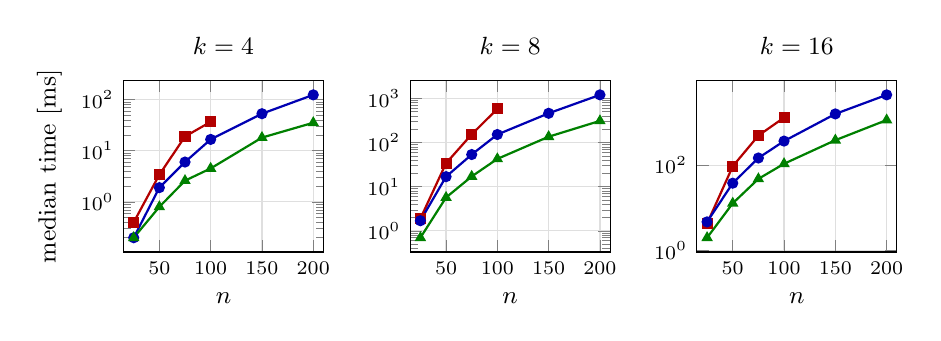
\begin{tikzpicture}
\begin{groupplot}[
  group style={group size=3 by 1, horizontal sep=1.1cm},
  width=0.34\textwidth, height=0.31\textwidth,
  ymode=log, xmin=15, xmax=210, xtick={50,100,150,200},
  xlabel={$n$}, grid=major, grid style={gray!25},
  tick label style={font=\scriptsize}, label style={font=\small},
  title style={font=\small}, legend style={font=\scriptsize, draw=none, fill=none},
  every axis plot/.append style={thick, mark size=1.6pt},
]
\nextgroupplot[title={$k=4$}, ylabel={median time [ms]}, legend to name=timelegend, legend columns=3]
\addplot[red!70!black, mark=square*] coordinates {(25,0.4)(50,3.4)(75,18.9)(100,36.6)};
\addlegendentry{TW DP}
\addplot[blue!70!black, mark=*] coordinates {(25,0.2)(50,1.9)(75,6.0)(100,16.6)(150,52.7)(200,122.9)};
\addlegendentry{capped DP}
\addplot[green!50!black, mark=triangle*] coordinates {(25,0.2)(50,0.8)(75,2.6)(100,4.5)(150,18.0)(200,35.1)};
\addlegendentry{certified}
\nextgroupplot[title={$k=8$}]
\addplot[red!70!black, mark=square*] coordinates {(25,1.9)(50,34.0)(75,153.9)(100,578.0)};
\addplot[blue!70!black, mark=*] coordinates {(25,1.7)(50,16.9)(75,53.6)(100,152.3)(150,460.4)(200,1203.9)};
\addplot[green!50!black, mark=triangle*] coordinates {(25,0.7)(50,5.7)(75,17.1)(100,42.7)(150,135.8)(200,310.0)};
\nextgroupplot[title={$k=16$}]
\addplot[red!70!black, mark=square*] coordinates {(25,4.3)(50,94.1)(75,493.4)(100,1300.8)};
\addplot[blue!70!black, mark=*] coordinates {(25,4.7)(50,37.9)(75,147.3)(100,366.7)(150,1587.0)(200,4434.8)};
\addplot[green!50!black, mark=triangle*] coordinates {(25,2.0)(50,12.8)(75,47.8)(100,107.9)(150,384.9)(200,1139.0)};
\end{groupplot}
\end{tikzpicture}

\pgfplotslegendfromname{timelegend}
\caption{Median solve time against $n$ on the scaling split, on a logarithmic scale
(data of \cref{tab:time}).}\label{fig:time}
\end{figure}

% ======================================================================
\section{Discussion and open problems}\label{sec:open}

The capped Delaunay dynamic program is simple. It uses only two integer predicates,
needs no geometric data structures, and improves the best deterministic worst-case
bound for $\log_2n\le k\le n^{o(1)}$. Our experiments suggest that, in practice, a
cheap greedy followed by one exact decision almost always suffices. We leave the
following questions open.
\begin{enumerate}[leftmargin=*]
\item Prove or refute \cref{conj:tight,conj:tree}. A proof of \cref{conj:tree}
  would give an $\Oh(2^kn^2k\log n)$ algorithm (\cref{prop:fpt}). Our counterexamples
  rule out the simpler variants based on alternation or on three-point seeds.
\item Is there an $o(n^3)$ algorithm for fixed $k\ge4$, matching the near-linear
  algorithm for $k=3$? Since $\mathrm{G}_k$ fails, a new characterisation is needed.
\item Can the factor $\log n$ of the binary search be removed, for instance by
  parametric search over the threshold representation of \cref{lem:thresholds}?
\end{enumerate}

\paragraph{Reproducibility.}
All code, data and scripts are available at \todo{repository URL or archived DOI}.
This includes the dataset generator, the experiment driver, the exact property
checkers, and the independent Python verification script.

% ======================================================================
\begin{thebibliography}{99}\small
\bibitem{Akagi18} T.~Akagi et~al.
  Exact algorithms for the max-min dispersion problem. In \emph{Proc.\ FAW 2018}, LNCS 10823, pp.~263--272, 2018.
\bibitem{BCKO08} M.~de~Berg, O.~Cheong, M.~van~Kreveld, M.~Overmars.
  \emph{Computational Geometry: Algorithms and Applications}, 3rd ed., Springer, 2008.
\bibitem{CD25} K.~Chen, A.~Dumitrescu. A couple of simple algorithms for $k$-dispersion. arXiv:2511.00692, 2025.
\bibitem{Del34} B.~Delaunay. Sur la sph\`ere vide. \emph{Bull.\ Acad.\ Sci.\ URSS}, 6:793--800, 1934.
\bibitem{Ede01} H.~Edelsbrunner. \emph{Geometry and Topology for Mesh Generation}. Cambridge University Press, 2001.
\bibitem{EG04} F.~Eisenbrand, F.~Grandoni. On the complexity of fixed parameter clique and dominating set.
  \emph{Theoretical Computer Science}, 326(1--3):57--67, 2004.
\bibitem{Gon85} T.~F.~Gonzalez. Clustering to minimize the maximum intercluster distance.
  \emph{Theoretical Computer Science}, 38:293--306, 1985.
\bibitem{Kob22} Y.~Kobayashi, S.-I.~Nakano, K.~Uchizawa, T.~Uno, Y.~Yamaguchi, K.~Yamanaka.
  An $O(n^2)$-time algorithm for computing a max-min 3-dispersion on a point set in convex position.
  \emph{IEICE Trans.\ Inf.\ \& Syst.}, E105-D(3), 2022.
\bibitem{NP85} J.~Ne\v{s}et\v{r}il, S.~Poljak. On the complexity of the subgraph problem.
  \emph{Commentationes Mathematicae Universitatis Carolinae}, 26(2):415--419, 1985.
\bibitem{RRT94} S.~S.~Ravi, D.~J.~Rosenkrantz, G.~K.~Tayi. Heuristic and special case algorithms for dispersion problems.
  \emph{Operations Research}, 42(2):299--310, 1994.
\bibitem{Shewchuk97} J.~R.~Shewchuk. Adaptive precision floating-point arithmetic and fast robust geometric predicates.
  \emph{Discrete \& Computational Geometry}, 18(3):305--363, 1997.
\bibitem{SBM26} V.~R.~Singireddy, M.~Basappa, J.~S.~B.~Mitchell. Algorithms for $k$-dispersion for points in convex position in the plane.
  \emph{Discrete Applied Mathematics}, 2026. Conference version in CALDAM 2023.
\bibitem{TW25} A.~Tkachenko, H.~Wang. Dominating set, independent set, discrete $k$-center, dispersion, and related problems for planar points in convex position.
  In \emph{Proc.\ STACS 2025}, LIPIcs 327, 73, 2025. arXiv:2501.00207.
\bibitem{TW26} A.~Tkachenko, H.~Wang. Maximum independent sets in disk graphs with disks in convex position.
  In \emph{Proc.\ SWAT 2026}, LIPIcs 370, 40, 2026. arXiv:2604.10828.
\bibitem{WK88} D.-W.~Wang, Y.-S.~Kuo. A study on two geometric location problems.
  \emph{Information Processing Letters}, 28(6):281--286, 1988.
\end{thebibliography}

\end{document}
